%%%%%%%%%%%%%%%%%%%%%%%%%%%%%%%%%%%%%%%%%
% Databases Report
%%%%%%%%%%%%%%%%%%%%%%%%%%%%%%%%%%%%%%%%%

%----------------------------------------------------------------------------------------
%	PACKAGES AND OTHER DOCUMENT CONFIGURATIONS
%----------------------------------------------------------------------------------------

\documentclass{article}

\usepackage{fancyhdr} % Required for custom headers
\usepackage{lastpage} % Required to determine the last page for the footer
\usepackage{extramarks} % Required for headers and footers
\usepackage[usenames,dvipsnames]{color} % Required for custom colors
\usepackage{graphicx} % Required to insert images
\usepackage{listings} % Required for insertion of code
\usepackage{courier} % Required for the courier font
\usepackage{enumitem}
\usepackage{titlesec}
\usepackage{csvsimple}
\usepackage{url}
\usepackage{etoolbox}
\patchcmd{\thebibliography}{\section*{\refname}}{}{}{}

% Margins
\topmargin=-0.45in
\evensidemargin=0in
\oddsidemargin=0in
\textwidth=6.5in
\textheight=9.0in
\headsep=0.25in

\linespread{1.1} % Line spacing

% Set up the header and footer
\pagestyle{fancy}
\fancyhead[LE,RO]{COMS20700\ Databases: Coursework 03}
\fancyhead[RE,LO]{}
\rfoot{Page\ \thepage\ of\ \protect\pageref{LastPage}} % Bottom right footer
\renewcommand\headrulewidth{0.4pt} % Size of the header rule
\renewcommand\footrulewidth{0.4pt} % Size of the footer rule

\setlength\parindent{0pt} % Removes all indentation from paragraphs

%----------------------------------------------------------------------------------------
%	CODE INCLUSION CONFIGURATION
%----------------------------------------------------------------------------------------

\definecolor{MyDarkGreen}{rgb}{0.0,0.4,0.0} % This is the color used for comments
\lstloadlanguages{Ruby}
\lstset{language=Ruby,
        frame=single, % Single frame around code
        basicstyle=\small\ttfamily, % Use small true type font
        keywordstyle=[1]\color{Blue}\bf, % Ruby functions bold and blue
        keywordstyle=[2]\color{Purple}, % Ruby function arguments purple
        keywordstyle=[3]\color{Blue}\underbar, % Custom functions underlined and blue
        identifierstyle=, % Nothing special about identifiers                                         
        commentstyle=\usefont{T1}{pcr}{m}{sl}\color{MyDarkGreen}\small, % Comments small dark green courier font
        stringstyle=\color{Purple}, % Strings are purple
        showstringspaces=false, % Don't put marks in string spaces
        tabsize=3, % 5 spaces per tab
        breaklines=true,
        morecomment=[l][\color{Blue}]{...}, % Line continuation (...) like blue comment
        numbers=left, % Line numbers on left
        firstnumber=1, % Line numbers start with line 1
        numberstyle=\tiny\color{Blue}, % Line numbers are blue and small
        %stepnumber=5 % Line numbers go in steps of 5
}

%----------------------------------------------------------------------------------------
%	DOCUMENT STRUCTURE COMMANDS
%----------------------------------------------------------------------------------------

\titlespacing\subsection{0pt}{1.0ex plus -1ex minus -.2ex}{-\parskip}
\setcounter{secnumdepth}{0} % Removes default section numbers
\newcounter{homeworkProblemCounter} % Creates a counter to keep track of the number of problems

\newcommand{\homeworkProblemName}{}
\newenvironment{homeworkProblem}[1][Question \arabic{homeworkProblemCounter}]{ % Makes a new environment called homeworkProblem which takes 1 argument (custom name) but the default is "Problem #"
\stepcounter{homeworkProblemCounter} % Increase counter for number of problems
\renewcommand{\homeworkProblemName}{#1} % Assign \homeworkProblemName the name of the problem
\subsection{\homeworkProblemName} % Make a section in the document with the custom problem count
}{}

\newcommand{\homeworkSectionName}{}
\newenvironment{homeworkSection}[1]{ % New environment for sections within homework problems, takes 1 argument - the name of the section
\renewcommand{\homeworkSectionName}{#1} % Assign \homeworkSectionName to the name of the section from the environment argument
}{}

%----------------------------------------------------------------------------------------
%	NAME AND CLASS SECTION
%----------------------------------------------------------------------------------------

\newcommand{\hmwkTitle}{Coursework\ 03 \\\vspace{0.5in} \Huge{Report}} % Assignment title
\newcommand{\hmwkClass}{\LARGE COMS20700\ Databases} % Course/class
\newcommand{\hmwkDueDate}{ May\ 18,\ 2014} % Due date

%----------------------------------------------------------------------------------------
%	TITLE PAGE
%----------------------------------------------------------------------------------------

\title{
\vspace{0.2in}
\textmd{\textbf{\hmwkClass:\ \hmwkTitle}}\\
\vspace{0.5in}
\textmd{\hmwkDueDate}
\vspace{1.5in}
}

\author{
  \textbf{Liban Abdulkadir}\\
  \texttt{la12808@my.bristol.ac.uk}\\
  \textbf{Ana Dumitra\c{s}}\\
  \texttt{ad12461@my.bristol.ac.uk}\\
  \textbf{Andra Irimia}\\
  \texttt{ai12821@my.bristol.ac.uk}\\
  \textbf{Ioan Troan\v{a}}\\
  \texttt{it12754@my.bristol.ac.uk}\\
\vspace{1in}
}

\date{}

%----------------------------------------------------------------------------------------

\begin{document}

\maketitle

%----------------------------------------------------------------------------------------
%	TABLE OF CONTENTS
%----------------------------------------------------------------------------------------

%\setcounter{tocdepth}{1} % Uncomment this line if you don't want subsections listed in the ToC

%\newpage
%\tableofcontents
%\newpage

%----------------------------------------------------------------------------------------
%	ABSTRACT
%----------------------------------------------------------------------------------------

\begin{abstract}
This report represents an outline of the Databases third coursework. The aim of this coursework is to design and implement, in a group of four, a database for an online multiplayer social gaming network similar to the Game Centre on iOS. \textbf{Section 1} includes a brief summary of our approach. In \textbf{Section 2} we mention what decisions and assumptions regarding the specification we have made. We then continue with detailing what the system we implemented can do (in \textbf{Section 3}), by going through the \texttt{SQL} statements requested by the client. \textbf{Section 4} discusses project management, while  \textbf{Section 5} approaches some future improvements.\textbf{Sections 6 and 7} include References and Appendices.

\end{abstract}

%----------------------------------------------------------------------------------------
%	Introduction
%----------------------------------------------------------------------------------------

\section{1  ~ Introduction}
\par {The goal of this coursework was to design and implement a database for a multiplayer social gaming network similar to the Game Centre on iOS. You can connect using a unique username and there will be displayed games that you can play with other users. Some games may feature achievements, where for completing a certain task, the player is rewarded points. Depending on the game, a leaderboard may be present where a player can compare his or her score with friends or with other players from around the world. The main features, however, were proposed by the client in the specification.} \\
\par {In order to accomplish this, we have decided to use \texttt {Postgre SQL} as a relational database management system. It runs on all major operating systems and it is easy to set up. Moreover, it is fully ACID compliant, having full support for custom types, arrays, foreign keys, joins, views, triggers and stored procedures. \cite{link1}}


%----------------------------------------------------------------------------------------
%	Design and Implementation
%----------------------------------------------------------------------------------------

\section{2 ~  Design and Implementation}
\subsection{Schema}
\par{By closely following the specification, we have created a database schema that would match the requirements as well as ease our work when retrieving data. For this purpose we have split the three main tables (Users, Games and Achievements) into 9 separate, smaller ones according to the normalisation rules. This way, we made sure that no many-to-many relations are present. We accomplished this by using a third junction table (or cross-reference table), say, AB with two one-to-many relationships A $\rightarrow$ AB and B $\rightarrow$ AB (for instance, table \texttt{ach} with two one-to-many relationships: \texttt{gameOwnAch} $\rightarrow$ \texttt{ach} and \texttt{gameAch} $\rightarrow$ \texttt{ach}).}\\

\par{The need to have a list of games each user owns required us to introduce a new table, \texttt{gameOwn}, that would have its own primary key and a foreign key to connect with the \texttt{user} table. Also, it will include the required fields \emph{rating, comment}, etc., as mentioned in Section A.2. of the specification.}\\

\par {In order to store which achievements the user has gained in a specific game, we have used a new table, \texttt{gameOwnAch}, that is linked with foreign keys to \texttt{gameOwn} and \texttt{ach}. A required attribute is \emph{dateAchieved}, which specifies when (date and time) the achievement was actually unlocked.}\\

\par {The \texttt{friend} table acts as a friends list with links between users and it can be used as follows: \emph{userId1} represents the id of the user that sent the request, while \emph{userId2} is the id of the user the request was sent to. An attribute named \emph{status} specifies if the status of the friend request and it is represented as a custom type that can take the values `accepted`, `rejected` or `awaiting`. The actual functionality is implemented in functions \texttt{send\_friend\_request(username1, username2, email)} and \texttt{friend\_request\_action(userame1, username2, action)}, that can be found in functions.sql. The first functions allows you (\emph{username1}) to send a request to another user that is identified by username (\emph{username2}) or e-mail address (\emph{email}). The action is then performed in the second function.}\\

\par{In order to provide one or more categories for each game we have created the \texttt{category} table, with fields name and rating (which specifies the age rating). Also, we decided to use a different table that would allow to have a ranking system within the genre/category. Therefore, we created table \texttt{gameCat} for this purpose, table that has a rank field, a primary key for identification and two foreign keys that link it with tables \texttt{category} and \texttt{game}. The table also allowed us to avoid a many-to-many relation.}\\

\par {The client specification mentions that one important feature of our system should be a leaderboard for each game, which shows the top 10 scores for that specific game. We have approached this by creating a function, \texttt{leaderboard(gameName)}, that, given a specific game, returns a view containing the usernames and the scores of the top 10 scores achieved for that game.}\\

\par {As mentioned in the specification, a maximum of 100 points per achievement is allowed. We have dealt with this by using a \emph{CHECK constraint} to limit the range that can be placed in column \emph{value} of table \texttt{gameAch}, 0 $\leq$ \emph{value} $\leq$ 100.}\\

\par {Two additional constraints were required to check the following:
\begin{itemize}[noitemsep, nolistsep]
  \item a maximum of 100 achievements per game,
  \item and a total maximum of 1000 points for all the achievements belonging to any particular game.
\end{itemize}
However, we have done this by creating a trigger \texttt{check\_gameAch()} that is automatically invoked when an \emph{INSERT event} occurs in table \texttt{GameAch}.}\\

\par {As we thought that users' \textsl{security} is important in a system like this, we decided to encrypt the users' passwords by storing the MD5 hash of the initial string (in hexadecimal). We implemented a trigger which checks each time a new user is created and also updates an existing user's password if it has been changed. This offers minimal security, since if someone would break into the database, the users' passwords cannot be easily decrypted and accounts will not be compromised.}\\

\par {See \emph{\textbf{Appendix A}} for the \textbf{ER Diagram} of our final database describing the various tables and their keys and showing how the entities/attributes are connected. In terms of data types of the columns used when creating the tables, we have used the \texttt{Postgre SQL} data types \cite{link2} as their proper use implies format validation of data and rejection of data outside the scope. A detailed list of the types used for each attribute can be found in \emph{\textbf{Appendix B}}.}\\

\subsection{Database dump}
\par {In order to test if the queries, functions and triggers we have written return the correct output, we have generated random data for each attribute of the relations. This has been done by generating fake data in \texttt{Ruby} using the \emph{Faker} \cite{link3} library. As we progressed through the questions, we realised there is a need of relations between data and that the ID randomness, for instance, prevented us from checking the accurateness of the queries' output. Changes also occurred when we had to introduce new attributes. \\ An example (the \texttt{category} table) can be seen below:}\\

%--------------- INSERT CODE HERE ---------------%
\lstinputlisting[language=Ruby]{insert_category.rb}

%----------------------------------------------------------------------------------------
%	Results and Evaluation
%----------------------------------------------------------------------------------------

\section{3 ~  Results and Evaluation}
 \par {After designing the system, creating tables with the triggers and functions mentioned above and populating them with dummy data, we were able to approach the queries and, this way, to add additional functionality to our system. A detailed explanation for each task can be found in this section. It is worth mentioning that the '...' in the resulting tables suggest that only part of the data was included in the report, for visualisation purposes.}
\vspace{5pt}

% Question 1
\begin{homeworkProblem}
\par {\textsl {Given a game, list all the users who own that game.}}
\vspace{5pt}
\par {For solving this question it is needed to select from the \texttt{gameOwn} table the IDs of all users who own the given game. Then from \texttt{user} are selected all usernames whose IDs are in the list resulted from the previous query.}\\\\
\texttt {SELECT q1('1');}

\begin{center}
    \begin{tabular}{| l | }
    \hline
    \textbf{q1}\\ \hline
    gilda\\ \hline
    mercedes\_hudson\\ \hline
    arden\\ \hline
    abelardo\\ \hline
    gaston\\ \hline
    kira.mohr\\ \hline
    annabelle.reilly\\ \hline
    liana\\ \hline
    linda\\ \hline
    haylee\\ \hline
    ignacio\\ \hline
    donald\_mohr\\ \hline
    godfrey.conn\\ \hline
    murl\\ \hline
    clair\\ \hline
    \end{tabular}
\end{center}
\end{homeworkProblem}

% Question 2
\begin{homeworkProblem}
\par {\textsl {Automatically update a game's average rating whenever a user adds or updates their rating for that game.}}
\vspace{5pt}
\par {We solve this question by implementing a \textsl{trigger}. Whenever an entry is updated or inserted into \texttt{gameOwn}, the average rating for the given game is recalculated. This is done by averaging all entries from \texttt{gameOwn} whose  \textsl{gameId} equals the ID of the game whose information was updated or inserted.}
\vspace{5pt}
\end{homeworkProblem}

% Question 3
\begin{homeworkProblem}
\par {\textsl {Change the database so that a game's average rating only appears if it has been rated by 10 or more users.}}
\vspace{5pt}
\par {Every time an entry is deleted or inserted into \texttt{gameOwn}, the table that links users with the games they own, it is needed to check if a game has been rated by at least 10 users. We assume that a user can rate a game only after he or she owns it.}
\vspace{5pt}
\end{homeworkProblem}

% Question 4
\begin{homeworkProblem}
\par {\textsl {Given a user and a game, display the user's score, rank on that game's leaderboard (even if they are outside the top 10) and an indication of where they appear relative to the average e.g. "85000 points - 1788 (Top 20\%)" or "13000 points - 16364 (Bottom 40\%)".}}
\vspace{5pt}
\par {Here}
\vspace{5pt}
\end{homeworkProblem}

% Question 5
\begin{homeworkProblem}
\par {\textsl {Create a list of the top 10 rated games in each genre/category.}}
\vspace{5pt}
\par {For this question, it is needed to compare the id of the \texttt{category} table with the id of the \texttt{gameCat} table to make sure they are a match, and also the \textsl{gameId} from \texttt{gameCat} to the actual \textsl{gameId}. It is then returned the category name, game name and rank for the top 10 games in the respective categories.}\\\\
\texttt{SELECT category.name, game.name, gameCat.rank FROM category, gameCat, game WHERE\\
    \-\ \-\ \-\ category.id = gameCat.catId AND\\
    \-\ \-\ \-\ gameCat.gameId = game.id AND\\
    \-\ \-\ \-\ gameCat.rank < 11\\
ORDER BY category.name, gameCat.rank;}
\begin{center}
    \begin{tabular}{| l | l | c|}
    \hline
    \textbf{category\_name} & \textbf{game\_name} & \textbf{rank} \\ \hline
    Baumbach, Dietrich and Kerluke & Hagenes, Koepp and Mohr & 1\\ \hline
    Baumbach, Dietrich and Kerluke & Gutkowski Group & 2\\ \hline
    Boyer-Bogisich & Hagenes, Koepp and Mohr & 1\\ \hline
    Boyer-Bogisich & Gutkowski Group & 2\\ \hline
    Cruickshank, Veum and Fisher & Goodwin, Windler and Morar & 1\\ \hline
    Cruickshank, Veum and Fisher & Gutkowski Group & 2\\ \hline
    Dach Inc & Gutkowski Group & 1\\ \hline
    Dach Inc & McKenzie LLC & 2\\ \hline
    Hane, OConner and RoweConner and RoweConner and Rowe & McKenzie LLC & 1\\ \hline
    Hane, OConner and RoweConner and RoweConner and Rowe & Mitchell-Sauer & 2\\ \hline
    Hartmann, Walker and Spencer & Goodwin, Windler and Morar & 1\\ \hline
    Hartmann, Walker and Spencer & Hagenes, Koepp and Mohr & 2\\ \hline
    ... & ... & ... \\ \hline
    \end{tabular}
\end{center}
\vspace{5pt}
\end{homeworkProblem}

% Question 6
\begin{homeworkProblem}
\par {\textsl {To help prevent cheating, add an optional maximum and minimum score value to each game and check that user's scores are within this range.}}
\vspace{5pt}
\par {To solve this question we have added two new attributes in the \texttt{game} table: \textsl{minimum} and \textsl{maximum}. The two new columns store for each game the minimum and maximum value of the score that a user can achieve. Every time a high score is updated we check if it is in the range: \textsl{minimum} $\leq$ \textsl{highScore} $\leq$ \textsl{maximum}. In case the score is too high or too low, an \textsl{exception} message will be displayed.}
\vspace{5pt}
\end{homeworkProblem}

% Question 7
\begin{homeworkProblem}
\par {\textsl {Add daily and weekly leaderboards for each game showing the best scores achieved this day or week.}}
\vspace{5pt}
\par {In order to complete this question, we wrote a \textsl{function} which takes as a parameter a string. If the string is 'weekly', then weekly leaderboards are returned; if it is 'daily', then the daily leaderboards are returned. A new field was added to the \texttt{gameOwn} table as it was needed the date the high score was achieved. The query checks the dates of these high scores and if they match the criteria, then they get displayed in a descending order.}\\\\
\texttt{SELECT * FROM q7('weekly') -- for weekly leaderbords}
\begin{center}
    \begin{tabular}{| l | l | c|}
    \hline
    \textbf{f\_game\_name} & \textbf{f\_user\_name} & \textbf{f\_highscore} \\ \hline
    Hagenes, Koepp and Mohr & gaston & 159\\ \hline
    Beatty-Swift & donald\_mohr & 156\\ \hline
    Heaney-Rice & gilda & 156\\ \hline
    Lynch-Thompson & mary\_shanahan & 148\\ \hline
    Waters, Strosin and Wunsch & faye\_emmerich & 146\\ \hline
    Bernier Group & maverick & 143\\ \hline
    Keebler, Bruen and Bartoletti & queenie.schneider & 142\\ \hline
    Williamson-Ortiz & maverick & 140\\ \hline
    Williamson-Ortiz & godfrey.conn & 140\\ \hline
    Osinski-Herzog & hildegard.walsh & 138\\ \hline
    ... &  ... & ... \\ \hline
    \end{tabular}
\end{center}

\texttt{SELECT * FROM q7('daily') -- for daily leaderbords}
\begin{center}
    \begin{tabular}{| l | l | c|}
    \hline
    \textbf{f\_game\_name} & \textbf{f\_user\_name} & \textbf{f\_highscore} \\ \hline
    Bernier Group & maverick & 143\\ \hline
    Howe-Eichmann & stephanie.batz & 136\\ \hline
    Mitchell-Sauer & arch & 131\\ \hline
    Kilback LLC & hildegard.walsh & 130\\ \hline
    Herman, Nikolaus and Ziemann & dameon & 120\\ \hline
    Ondricka, Kreiger and Trantow & matilda\_dare & 117\\ \hline
    Sanford and Sons & jed.ko & 112\\ \hline
    Torp and Sons & hugh.towne & 107\\ \hline
    Williamson-Ortiz & jed.ko & 102\\ \hline
    Lynch-Thompson & al & 100\\ \hline
    ... &  ... & ... \\ \hline
    \end{tabular}
\end{center}
\end{homeworkProblem}

% Question 8
\begin{homeworkProblem}
\par {\textsl {Check new usernames against a list of obscene or offensive terms (if possible check for substrings as well as the whole name). If such a username exists, lock the account.}}
\vspace{5pt}
\par {When a user creates a new account, its username is automatically checked against a list of obscene or offensive words. If the username matches any of the words, the account will be deleted. We assumed locking the account means deleting the entry from the \texttt{user} table.}
\vspace{5pt}
\end{homeworkProblem}

% Question 9
\begin{homeworkProblem}
\par {\textsl {The client wants to add a 'Hot List' which shows the 10 games, which have been played most often in the past week – add the necessary fields, tables, queries, triggers and/or procedures to achieve this.}}
\vspace{5pt}
\par {In order to find the most played games, we required a table that would hold the game play times (when a game starts) for each game. Therefore, we created \texttt{gameTime}, which has the\textsl{gameOwnId} and the \textsl{playedOn} timestamp as fields. We then calculated the count of gameplay dates in the past week and this way, were able to make a 'Hot List' which shows the most played games in that specific week.}\\\\
\texttt{SELECT game.name, COUNT(gameTime.playedOn::date) FROM game, gameOwn, gameTime WHERE\\
   \-\ \-\ \-\ game.id = gameOwn.gameId AND\\
   \-\ \-\ \-\ gameTime.gameOwnId = gameOwn.id AND\\
   \-\ \-\ \-\ gameTime.playedOn::date >= (current\_date - integer '7') AND\\
   \-\ \-\ \-\ gameTime.playedOn::date <= current\_date\\
   \-\ \-\ \-\ GROUP BY game.name\\
   \-\ \-\ \-\ ORDER BY COUNT(gameTime.playedOn) DESC\\
LIMIT 10;}

\begin{center}
    \begin{tabular}{| l | c |}
    \hline
    \textbf{name} & \textbf{count}\\ \hline
    Kilback LLC & 175\\ \hline
    Lynch-Thompson & 166\\ \hline
    Price Inc & 160\\ \hline
    Moore Group & 156\\ \hline
    Heaney-Rice & 150\\ \hline
    Hagenes, Koepp and Mohr & 143\\ \hline
    Wiza, Daugherty and Rowe & 141\\ \hline
    Howe-Eichmann & 130\\ \hline
    Dietrich, Altenwerth and Bins & 127\\ \hline
    Kuhlman-Kemmer & 127\\ \hline
    \end{tabular}
\end{center}
\vspace{5pt}
\end{homeworkProblem}

% Question 10
\begin{homeworkProblem}
\par {\textsl {The client wants to allow users to send friend requests to other users using their username or email address. What additional fields/tables would you need to add to allow for this functionality? You will need to keep track of the request, the response (if any) and some way of keeping track of user friends lists. If possible, extend this system to allow users to send an invite to a friend to play a particular game.}}
\vspace{5pt}
\par {Here}
\vspace{5pt}
\end{homeworkProblem}

% Question 11
\begin{homeworkProblem}
\par {\textsl {Given a user and a game, show a leaderboard which lists just the user and their friends.}}
\vspace{5pt}
\par {Here}
\vspace{5pt}
\end{homeworkProblem}

% Question 12
\begin{homeworkProblem}
\par {\textsl {List all of a user's friends and show whether they are currently logged on. If they are not logged on, show when they were last logged on and what they were playing.}}
\vspace{5pt}
\par {Here}
\vspace{5pt}
\end{homeworkProblem}

% Question 13
\begin{homeworkProblem}
\par {\textsl {Given a user and a game, show how many achievements they've got (out of how many in total the game has) and how many points worth of achievements they have for that game e.g. "16 of 80 achievements (95 points)".}}
\vspace{5pt}
\par {We wrote a function that, given a user and a game id, returns how many achievements the user has unlocked out of how many the game has and also how many points those achievements are worth. The game id is used instead of the game name because in the database there might be more than one version of the same game. In order to return the required message, it is first needed to check how many achievements the given game has and then count the number of achievements the user has unlocked for that particular game. In order to obtain the number of points those achievements are worth, we count the value of all achievements the user has unlocked.}\\\\
\texttt {SELECT show\_achievements('gilda', 1);\\
"1 of 1 achievements (18 points)"}
\vspace{5pt}
\end{homeworkProblem}

% Question 14
\begin{homeworkProblem}
\par {\textsl {Show a status screen for the player showing their username, status line, number of games owned, total number of achievement points and total number of friends.}}
\vspace{5pt}
\par {To solve this task, we first wrote a \textsl{query} to find the username, status line and the number of games owned. Afterwards, we wrote a similar query but for the number of achievement points and the number of friends. Following this, we merged the 2 tables into one, this way displaying all the required values. This was aquired by using an inner join on the username.
In the end, we moved the queries into a \textsl{function} in order to allow the user to specify the user id he/she requires information for.}\\\\
\texttt{SELECT * FROM q14(11);}
\begin{center}
    \begin{tabular}{| l | c | c | c | c | }
    \hline
    \textbf{n\_username} & \textbf{n\_status} & \textbf{n\_games} & \textbf{n\_ach\_points} & \textbf{n\_friends}\\ \hline
    yvonne & ut maiores quibusdam ducimus labore illum ... & 2 & 6410 &5 \\ \hline
    \end{tabular}
\end{center}
\vspace{5pt}
\end{homeworkProblem}

% Question 15
\begin{homeworkProblem}
\par {\textsl {Given a user and a game, list the achievements for that game (apart from ones which have the hidden flag set and the user hasn't earned). They should be listed with ones the player has earned listed first. For each achievement, list the title, points, description (which will vary depending on whether the player has earned that title or not) and when the achievement was earned.}}
\vspace{5pt}
\par {For this question we used \textsl{functions} in order to allow the user to specify the exact username and game he requires information for. We select from the database the achievement title, value, description (which depends on whether the achievement was earned or not) and the date the achievement was earned. In order to return the correct result, it was needed to perform a number of checks on the achievements: if the achievement can be shown or not, if the achievement belongs to that game, that user and so on. At the end, the results were ordered by the date they were achieved.}\\\\
\texttt{SELECT * FROM q15(1, 13);}
\begin{center}
    \begin{tabular}{| l | c | l | l | }
    \hline
    \textbf{f\_ach\_title} & \textbf{f\_ach\_value} & \textbf{f\_description} & \textbf{f\_date\_achieved}\\ \hline
    Regional Usability Supervisor & 26 & ["Sit est esse nihil."] & 2012-01-25 00:00:00+00\\ \hline
    Internal Solutions Administrator & 12 & ["Labore officia  ..."] & 2012-07-05 00:00:00+01\\ \hline
    Principal Accountability Executive & 63 & ["Earum consec ..."] & 2013-02-21 00:00:00+00\\ \hline
    Global Implementation Representative & 51 & ["Molestiae vero  ..."] & 2013-07-02 00:00:00+01\\ \hline
    Corporate Security Planner & 21 & ["Nemo magni  ..."] & 2013-10-27 00:00:00+01\\ \hline
    \end{tabular}
\end{center}
\vspace{5pt}
\end{homeworkProblem}

% Question 16
\begin{homeworkProblem}
\par {\textsl {Given a user and a named friend, for each game they both own, list the name of the game and the number of achievement points each of the users has for that game. If possible, at the end of that list add all the games that are owned by only one of the two users, showing how many points they have and a blank for the other user.}}
\vspace{5pt}
\par {To solve this question we first find the games owned by each user and store them in separate tables. For each of the two users we have a table that has the IDs of the games they own and the total number of achievements they unlocked for each game. In order to find the common games for the two users, we apply an inner join on the two tables mentioned above. The resulted table only has the IDs of the games owned by both users and the number of achievements each user has unlocked. At the end of the table are appended the games only owned by the first user by selecting from the table that stores the games owned by the first user the ones that are not in the common table. We do the same for the games owned only by the second user. We update the resulted table with the name of each game based on their ID. The table now stores the ID of each game, its name, and the total achievements unlocked by each of the two users. The \textsl{function} will only return the last 3 attributes of the resulted table. If a user does not own the game, then the achievement column will have value 0; same if the user has not unlocked any achievements for a game they own.}\\\\
\texttt {SELECT * FROM common\_games('jarod\_ledner', 'yvonne');}

\begin{center}
    \begin{tabular}{| l | c | c | }
    \hline
    \textbf{game\_name} & \textbf{no\_achievements1} & \textbf{no\_achievements2}\\ \hline
    Wisoky and Sons & 298 & 276\\ \hline
    Gutkowski Group & 436 & 0\\ \hline
    Wolff Group & 406 & 0\\ \hline
    Wiza, Daugherty and Rowe & 297 & 0\\ \hline
    Keebler, Bruen and Bartoletti & 367 & 0\\ \hline
    Kuhlman-Kemmer & 193 & 0\\ \hline
    Hagenes, Koepp and Mohr & 431 & 0\\ \hline
    Howe-Eichmann & 0 & 284\\ \hline
    \end{tabular}
\end{center}
\end{homeworkProblem}

% Question 17
\begin{homeworkProblem}
\par {\textsl {The client has realised that for some games (e.g. golf, driving games) lower scores are better. They want to add a "sort order" flag to the game to indicate this. They've also realised that many games have a format other than simply points when displaying scores. Add a "score format" field (e.g. int, time, money) to the Game table. The sort order and score format should be taken into account when displaying leaderboards.}}
\vspace{5pt}
\par {For this question we implemented two new types for \texttt{game} table: the sort order and score format. Sort order can be ascending or descending, depending on the game and score format can be int, time, money or any other currency relevant to the game. Both types are now taken into account when displaying new leaderboards.}
\vspace{5pt}
\end{homeworkProblem}

% Question 18
\begin{homeworkProblem}
\par {\textsl {Suggest another user as a friend, if they have a number of friends and/or games in common with the user. You should show the name of the potential friend and how many games/friends they have in common with the user.}}
\vspace{5pt}
\par {Here}
\vspace{5pt}
\end{homeworkProblem}

% Question 19
\begin{homeworkProblem}
\par {\textsl {Automatically suggest a game, which a user might be interested in. Games should only be suggested if the user doesn't already own them. Suggestions could be made on the basis that other users who make similar ratings also rate this item highly (though you may use another recommendation metric if you prefer).}}
\vspace{5pt}
\par {Here}
\vspace{5pt}
\end{homeworkProblem}

% Question 20
\begin{homeworkProblem}
\par {\textsl {Write another query/trigger/procedure of your choice, which really shows off what your database can do.}}
\vspace{5pt}
\par {For this part we have decided to change the way a user's highscore is updated depending on their in-game rank. This was achieved by splitting all players for each game into 4 different groups of equal size when ordered by their rank. This means that the top 25\% percent are in the first group and so on. Whenever the highscore is increased, a multiplier is applied to the difference. The multiplier is defined as follows:}
\vspace{5pt}
\begin{center}
    \begin{tabular}{| c | c |}\hline
    \textbf{Group} & \textbf{Multiplier} \\ \hline
    1 & 0.4 \\ \hline
    2 &  0.8 \\ \hline
    3 & 1.2 \\ \hline
    4 & 1.4 \\  \hline
    \end{tabular}
\end{center}
\par {This ensures that players at the top of the leaderboard will find it harder to increase their score even further.}
\end{homeworkProblem}

%----------------------------------------------------------------------------------------
%	Project Management
%----------------------------------------------------------------------------------------

\section{4 ~  Project Management}
\par {This project was divided, even from the beginning, into the following stages:
\begin{enumerate}[noitemsep,nolistsep]
  \item Database design and E/R Diagram
  \item Scripts for dummy data
  \item Tables creation
  \item Queries, Triggers and Functions for the given tasks
  \item Report
\end{enumerate}}
\vspace{6pt}
\par {We worked all together when designing the database in order to make sure that everyone is aware and agrees with the decisions we took. One of the team members then easily designed the \textsl {E/R Diagram} using the \texttt{Gliffy} online tool.}\\
 
\par {After that, we split the tasks among us, starting with the scripts for dummy data and then spending the most time on concurrently implementing the required features of our system. During development, we encountered questions which required us to slightly change the database, having to update the \textsl{E/R Diagram} and the scripts. For this stage we have used \texttt{Trello}, an online kanban board, which allowed us to know the state of the project at any point and to make sure that we are not working on the same task, at the same time.}\\
 
\par {For version control we have decided to use git due to the team members' familiarity with the tool and a free private git repository on \texttt{GitHub}. Each of us worked on a separate branch, sending pull requests when done with a task. This way we made sure that the master branch only contained code that was reviewed and tested by at least one member of the team.}\\

\par {\texttt{Google Docs} allowed us, as a team, to contribute in real time to the report. This constituted a draft, the main report being written in \LaTeX.}

%----------------------------------------------------------------------------------------
%	Future improvements
%----------------------------------------------------------------------------------------

\section{5 ~  Future improvements}
\par {}
\par {In terms future improvements, it is worth mentioning that here are a number of attributes in our database that are not being used at the moment. For instance, the \texttt{category} table stores the age rating. This can be used in restricting access to certain users if their age is below a given value. In order to do this, however, we will also need to know the user's age, so we will need to add another column to the \texttt{user} table that will store the age or date of birth. Although we are not using some of the attributes, we decided to keep them in the database so it will be easier to add extra features to the system. }

%----------------------------------------------------------------------------------------
%	References
%----------------------------------------------------------------------------------------

\section{6 ~ References}
In addition to the lecture slides, we have used the following resources in order to fully understand the concepts used in this assignment and to be able to easily work with PostgreSQL:
\nocite{link4, link5, link6, db}
\bibliographystyle{plain}
\bibliography{report}

%----------------------------------------------------------------------------------------
%	Appendices
%----------------------------------------------------------------------------------------
\newpage
\section{7 ~ Appendices}
\appendix

\chapter{\textbf{Appendix A: ER Diagram}}
\begin{center}
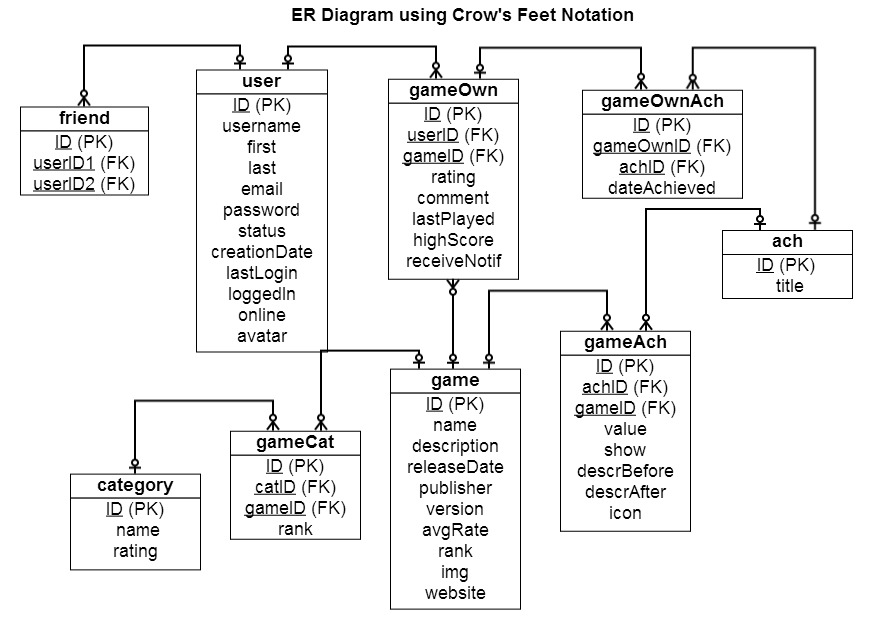
\includegraphics[width=0.80\columnwidth]{er} % Import image
\end{center}

\chapter{\textbf{Appendix B: Data Types}}
\begin{center}
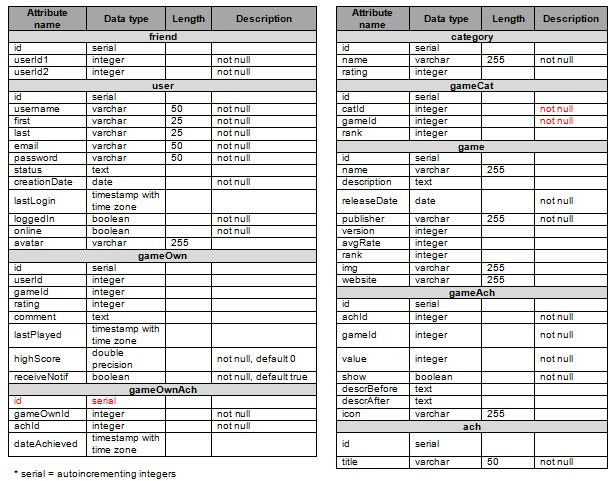
\includegraphics[width=0.87\columnwidth]{types} % Import image
\end{center}

\chapter{\textbf{Appendix C: Mark Allocation}}
\begin{flushleft}
    \begin{tabular}{| l | c |}
    \hline
    \textbf{Name} & \textbf{Allocated Mark}\\ \hline
    Liban Abdulkadir & 0.25\\ \hline
    Ana Dumitra\c{s} & 0.25 \\ \hline
    Andra Irimia & 0.25 \\ \hline
    Ioan Troan\v{a} & 0.25 \\ \hline
    \end{tabular}
\end{flushleft}

\end{document}
